\documentclass[11pt,letterpaper]{article}

% ------------------------------------------------------------------
% Packages
% ------------------------------------------------------------------
\usepackage[margin=1in]{geometry}
\usepackage[T1]{fontenc}

\usepackage{mathpazo}
\usepackage[scaled=0.92]{helvet}
\usepackage{microtype}
\usepackage{amsmath}
\usepackage{graphicx}
\usepackage{booktabs}
\usepackage{longtable}
\usepackage{array}
\usepackage{tabularx}
\usepackage{float}
\usepackage[font=small,labelfont=bf]{caption}
\usepackage{xcolor}
\usepackage{tikz}
\usetikzlibrary{arrows.meta,positioning}
\usepackage{enumitem}
\usepackage[hidelinks]{hyperref}

\definecolor{accent}{HTML}{1F3A5F}
\definecolor{boxbg}{HTML}{EEF3F9}
\newcommand{\repourl}{\url{https://github.com/98DanPazos/doac-cua-ontario}}

\setlist{itemsep=2pt,topsep=4pt}
\graphicspath{{figures/}}

% Keep the report compilable when optional figures have not been supplied.
\newcommand{\safeincludegraphics}[2][]{%
  \IfFileExists{#2}{\includegraphics[#1]{#2}}{%
    \fbox{\parbox[c][3cm][c]{0.85\linewidth}{\centering
      Missing figure: \texttt{\detokenize{#2}}\\[4pt]
      Add the image file to the figures folder to display it.}}}%
}

\title{\textbf{Generic Apixaban Versus Warfarin for Stroke Prevention\\in Non-Valvular Atrial Fibrillation}\\[4pt]
\large A Cost-Utility and Budget Impact Analysis from the Perspective of\\the Ontario Public Drug Programs}
\author{Daniel Pazos Cordero\\[2pt]
\small M.Sc. Applied Economics (Banking and Financial Markets), University of Bath}
\date{October 2026}

\begin{document}
\maketitle

\begin{center}
\fcolorbox{accent}{boxbg}{\parbox{0.92\textwidth}{\small
\textbf{About this report.} This is an independent portfolio project prepared to demonstrate
health economic modelling methods. It is not affiliated with, reviewed by, or endorsed by
Canada's Drug Agency (CDA-AMC). It adapts the structure and inputs of the published CADTH
worked example \cite{cadthwe} and should not be used to inform clinical or funding decisions.
Developed with AI assistance under author direction; all analytical choices, inputs, and results
reviewed and validated by the author.
}}
\end{center}

% ==================================================================
\section*{Executive Summary}
% ==================================================================

\textbf{Decision problem.} Direct oral anticoagulants (DOACs) were assessed by CADTH in
2012--2013 when they were available only as branded products. Generic apixaban is now listed
on the Ontario Drug Benefit (ODB) Formulary at \$0.4084 per 5\,mg tablet, 75\% below the
brand price of \$1.6336. This report asks whether generic entry changes the value of apixaban
relative to warfarin for publicly funded patients with non-valvular atrial fibrillation (AF).

\textbf{Methods.} A five-state cohort Markov model with three-month cycles followed patients
aged 70 with a CHADS\textsubscript{2} score of 2 over a lifetime horizon. Clinical inputs,
utilities and event costs were taken from the CADTH 4th-edition guidelines worked example
\cite{cadthwe}; costs were inflated to 2025 Canadian dollars and drug prices updated to the
October 2026 ODB Formulary. The analysis followed the CADTH reference case: public health
care payer perspective, 1.5\% annual discounting of costs and quality-adjusted life-years
(QALYs), and probabilistic analysis with 5,000 simulations.

\textbf{Results.}
\begin{itemize}
  \item Generic apixaban was \textbf{dominant}: it cost \$5,608 less per patient and produced
        0.236 more QALYs than warfarin (probabilistic: $-\$5{,}589$, 95\% CI $-\$8{,}352$ to
        $-\$3{,}242$; 0.236 QALYs, 95\% CI 0.127 to 0.359).
  \item Apixaban was cost-saving and more effective in \textbf{100\%} of 5,000 probabilistic
        simulations. At the brand price, it was cost-saving in only 13.8\%.
  \item Apixaban remains cost-saving up to \textbf{\$1.41 per tablet}, 3.4 times the current
        generic price, and cost-effective at \$50,000 per QALY up to \$3.51 per tablet.
  \item The conclusion held in every one-way sensitivity analysis and in all ten scenario
        analyses, including setting every apixaban treatment effect to the upper bound of its
        95\% confidence interval.
  \item Switching an estimated 16,500 remaining warfarin users aged 65+ over three years would
        cost the drug plan about \$6.0 million in drug costs but save the wider health system
        about \$11.3 million.
\end{itemize}

\textbf{Conclusion.} At current Ontario prices, generic apixaban is expected to be both less
costly and more effective than warfarin for stroke prevention in non-valvular AF.

\newpage
\tableofcontents
\newpage

% ==================================================================
\section{Introduction and Rationale}
% ==================================================================

\subsection{Clinical context}

Atrial fibrillation is the most common sustained cardiac arrhythmia and increases the risk of
ischaemic stroke roughly fivefold. Oral anticoagulation is the mainstay of stroke prevention.
For decades the standard option was warfarin, a vitamin K antagonist that is inexpensive to
buy but requires regular International Normalized Ratio (INR) blood testing, has many drug and
food interactions, and carries a substantial risk of intracranial haemorrhage (ICH).

The DOACs (dabigatran, rivaroxaban, apixaban and edoxaban) were compared with warfarin in large
randomised trials. In ARISTOTLE, apixaban 5\,mg twice daily reduced stroke or systemic embolism
(hazard ratio [HR] 0.79, 95\% CI 0.66--0.95), major bleeding (HR 0.69, 95\% CI 0.60--0.80),
haemorrhagic stroke (HR 0.51) and all-cause death (HR 0.89, 95\% CI 0.80--0.99)
\cite{aristotle}.

\subsection{Why revisit the economics now}

CADTH's 2012 therapeutic review of the new oral anticoagulants \cite{wells2012} and the
economic evaluation underlying it \cite{coyle2013} were conducted when apixaban cost about
\$1,289 per year. At that price, apixaban cost more than warfarin and was judged cost-effective
because its health gains justified the additional spending: an incremental cost-effectiveness
ratio (ICER) of \$22,875 per QALY versus warfarin in patients with a CHADS\textsubscript{2} score
of 2 \cite{cadthwe}.

Generic apixaban is now widely available. The ODB Formulary lists interchangeable generic
apixaban 5\,mg products at \$0.4084 per tablet, compared with \$1.6336 for brand Eliquis
\cite{odb}. The annual drug cost has fallen from roughly \$1,193 (2026 brand
list price) to \$298, which is now below the combined annual cost of warfarin and INR monitoring
(about \$384). When a comparator's price changes this much, the previous economic conclusion
needs updating: the question is no longer whether apixaban's benefits justify its extra cost,
but whether it still costs extra at all.

\subsection{Objectives}

\begin{enumerate}
  \item Estimate the cost-utility of generic apixaban versus warfarin at current Ontario prices,
        following the CADTH reference case \cite{cadthguide}.
  \item Characterise parameter and structural uncertainty through probabilistic, one-way and
        scenario analyses.
  \item Identify the apixaban price thresholds at which the conclusion would change.
  \item Estimate the three-year budget impact of switching remaining warfarin users in Ontario.
\end{enumerate}

% ==================================================================
\section{Methods}
% ==================================================================

\subsection{Decision problem}

Table~\ref{tab:pico} summarises the decision problem and the main features of the analysis.

\begin{table}[H]
\centering
\caption{Decision problem and reference-case specification}
\label{tab:pico}
\small
\begin{tabularx}{\textwidth}{@{}lX@{}}
\toprule
Element & Specification \\
\midrule
Population & Adults with non-valvular AF requiring anticoagulation; reference cohort aged 70 with
             CHADS\textsubscript{2} = 2 \\
Intervention & Generic apixaban 5\,mg twice daily \\
Comparator & Warfarin, dose-adjusted to INR 2.0--3.0, with INR monitoring \\
Outcomes & QALYs, life-years, strokes, ICH, major bleeds; costs in 2025 CAD \\
Type of evaluation & Cost-utility analysis; supplementary cost comparison and budget impact \\
Perspective & Publicly funded health care payer (Ontario) \\
Time horizon & Lifetime (to age 100); scenarios at 2 and 10 years \\
Discounting & 1.5\% per year on costs and QALYs; scenarios at 0\% and 3\% \\
Model & Cohort Markov model, five health states, three-month cycles \\
Software & Python 3.11 (NumPy, pandas, Matplotlib) \\
\bottomrule
\end{tabularx}
\end{table}

\subsection{Model structure}

The model (Figure~\ref{fig:structure}) follows a cohort through five health states. All
patients start in \textbf{S0} (AF, no prior event), receiving the assigned anticoagulant. In
each three-month cycle, patients may die of non-vascular causes or experience one clinical
event: stroke, ICH, major extracranial bleed, myocardial infarction (MI), transient ischaemic
attack (TIA) or minor bleed. Following the CADTH worked example \cite{cadthwe}, patients who
survive a stroke, ICH or major bleed discontinue anticoagulation and continue on aspirin.

\begin{figure}[H]
\centering
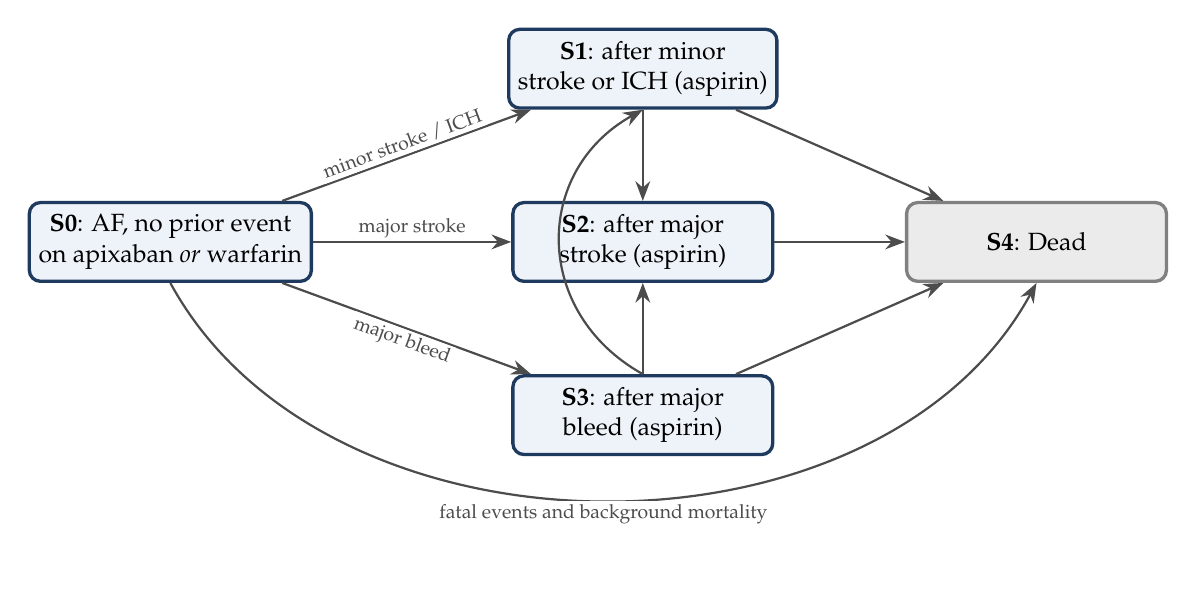
\begin{tikzpicture}[
  state/.style={draw=accent, very thick, rounded corners, fill=boxbg, minimum width=3.3cm,
                minimum height=1cm, align=center, font=\small},
  arr/.style={-{Stealth[length=2.5mm]}, thick, color=black!70},
  lab/.style={font=\scriptsize, fill=white, inner sep=1pt}]
  \node[state] (s0) at (0,0) {\textbf{S0}: AF, no prior event\\on apixaban \emph{or} warfarin};
  \node[state] (s1) at (6,2.2) {\textbf{S1}: after minor\\stroke or ICH (aspirin)};
  \node[state] (s2) at (6,0) {\textbf{S2}: after major\\stroke (aspirin)};
  \node[state] (s3) at (6,-2.2) {\textbf{S3}: after major\\bleed (aspirin)};
  \node[state, fill=black!8, draw=black!50] (d) at (11,0) {\textbf{S4}: Dead};
  \draw[arr] (s0) -- node[lab, sloped, above] {minor stroke / ICH} (s1);
  \draw[arr] (s0) -- node[lab, above] {major stroke} (s2);
  \draw[arr] (s0) -- node[lab, sloped, below] {major bleed} (s3);
  \draw[arr] (s1) -- (s2);
  \draw[arr] (s3) -- (s2);
  \draw[arr] (s3.north) .. controls (4.6,-0.9) and (4.6,0.9) .. (s1.south);
  \draw[arr] (s1) -- (d);
  \draw[arr] (s2) -- (d);
  \draw[arr] (s3) -- (d);
  \draw[arr] (s0.south) .. controls (2,-4.2) and (9,-4.2) .. node[lab, below] {fatal events and background mortality} (d.south);
\end{tikzpicture}
\caption{Model structure. Each living state can also remain in place. TIA, minor bleeds and
non-fatal MI generate costs and QALY losses in the cycle they occur but do not change state.}
\label{fig:structure}
\end{figure}

The five-state structure is a deliberate simplification of the 173-state model used in the
worked example. It keeps the events that drive costs and outcomes in this decision (stroke
severity, ICH and major bleeding) while remaining fully auditable. The consequences of this
simplification are examined in the validation (Section~\ref{sec:validation}).

\subsection{Transition probabilities}

Event inputs are annual probabilities $p$ observed in the warfarin arm of RE-LY
\cite{rely} for CHADS\textsubscript{2} = 2, as reported in the worked example. Each was converted
to a rate, adjusted, and converted back to a probability for the cycle length
$\Delta t = 0.25$ years:
\begin{equation}
r = -\ln(1-p), \qquad
r' = r \times \text{RR}_{\text{age}} \times \text{RR}_{\text{history}} \times \text{RR}_{\text{aspirin}},
\qquad
p_{\text{cycle}} = 1 - e^{-r'\Delta t}.
\end{equation}
Stroke risk was increased by a factor of 1.5 per decade of age above 70, by 2.2 after a
previous stroke or ICH, and by the aspirin-versus-warfarin relative risk in states S1--S3.

The effect of apixaban was applied in S0 only, using odds ratios (OR) from the CADTH network
meta-analysis \cite{wells2012}:
\begin{equation}
p_{\text{apixaban}} = \frac{\text{OR}\cdot p_{\text{warfarin}}}{1 - p_{\text{warfarin}} + \text{OR}\cdot p_{\text{warfarin}}}.
\end{equation}
Odds ratios were 0.79 for stroke, 0.42 for ICH, 0.80 for major bleeding and 0.88 for MI. These
are consistent with, and slightly more conservative than, the ARISTOTLE estimates for bleeding
\cite{aristotle}.

Background (non-vascular) mortality was anchored to the RE-LY rate at age 70 (3.3\% per year)
and increased with age following the gradient of the Statistics Canada 2021--2023 life table
\cite{statcanlt}. A Gompertz curve, $\ln q_x = -11.358 + 0.1046x$, was fitted to the life-table
probabilities at ages 70--90 to provide a smooth age gradient. Mortality was multiplied by 2.3
after a stroke.

\subsection{Health-state utilities}

Utilities were taken from the worked example \cite{cadthwe}: 0.81 for AF without prior events,
0.75 after a minor stroke or ICH, and a weighted average of 0.39 (modified Rankin 3--4) and 0.11
(Rankin 5) after a major stroke. Utility declined by 0.00029 per year of age above 70. One-off
decrements were applied for MI (0.125), major bleed (0.092), TIA (0.103) and minor bleed (0.013)
in the cycle of the event.

\subsection{Resource use and costs}

Costs reflect a public payer perspective in 2025 Canadian dollars (Table~\ref{tab:costs}). Event
and long-term health-state costs from the worked example (2011 CAD) were inflated using the
all-items Consumer Price Index (164.2/119.9 = 1.3695) \cite{statcancpi}. Drug costs used current
ODB unit prices without inflation, since generic prices do not track general inflation. Dispensing
fees and mark-ups were excluded, consistent with CDA-AMC practice.

\begin{table}[H]
\centering
\caption{Key cost inputs (2025 CAD)}
\label{tab:costs}
\small
\begin{tabular}{@{}lrl@{}}
\toprule
Item & Value & Source \\
\midrule
Generic apixaban 5\,mg twice daily, per year & \$298 & ODB, Oct 2026 \cite{odb} \\
Brand apixaban (Eliquis) 5\,mg twice daily, per year & \$1,193 & ODB, Oct 2026 \cite{odb} \\
Warfarin 5\,mg daily, per year & \$55 & \cite{cadthwe} (2011 ODB) \\
INR monitoring, per year & \$330 & \cite{cadthwe} $\times$ CPI \\
Aspirin, per year & \$39 & \cite{cadthwe} (2011 ODB) \\
Major stroke, acute & \$77,874 & \cite{cadthwe} $\times$ CPI \\
Minor or fatal stroke, acute & \$23,007 & \cite{cadthwe} $\times$ CPI \\
Intracranial haemorrhage & \$22,677 & \cite{cadthwe} $\times$ CPI \\
Major bleed & \$6,015 & \cite{cadthwe} $\times$ CPI \\
Long-term care after major stroke, per year & \$26,115 & \cite{cadthwe} $\times$ CPI \\
Long-term care after minor stroke or ICH, per year & \$10,813 & \cite{cadthwe} $\times$ CPI \\
\bottomrule
\end{tabular}
\end{table}

\subsection{Model validation}
\label{sec:methods-validation}

Following the worked example's validation approach \cite{cadthwe}, the model was assessed in two
ways:
\begin{enumerate}
  \item \textbf{Cross-validation.} Re-running the model with the worked example's 2011 costs and
        brand apixaban price, and comparing outputs with the published results for
        CHADS\textsubscript{2} = 2.
  \item \textbf{Internal validity.} (a) Setting all utilities to 1 and removing decrements must
        make QALYs equal life-years. (b) Setting all apixaban odds ratios to 1 and equalising drug
        costs must make the two arms identical. (c) Lowering the stroke odds ratio must increase
        QALYs monotonically. (d) Raising the discount rate must lower discounted QALYs. Mass balance
        (state occupancy summing to 1) was checked in every cycle.
\end{enumerate}

\subsection{Analysis of uncertainty}

\textbf{Probabilistic analysis.} Following the worked example's conventions, probabilities and
utilities were assigned beta distributions, odds ratios and relative risks lognormal distributions
based on their 95\% confidence intervals, event costs gamma distributions with a 25\% coefficient
of variation, and utility decrements normal distributions. Drug prices were fixed. Expected values
were estimated from 5,000 Monte Carlo simulations with a fixed random seed. The same simulations
were repeated at the brand apixaban price to isolate the effect of generic entry.

\textbf{One-way sensitivity analysis.} Each of the 50 parameters was set to its low and high
values (Appendix~\ref{app:params}) while all others were held at base values. Results are reported
as incremental net monetary benefit (INMB) at \$50,000 per QALY, since ICERs are not meaningful
when one option dominates.

\textbf{Scenario analyses.} Scenarios addressed methodological and structural uncertainty:
discount rates of 0\% and 3\%, time horizons of 2 and 10 years, waning of the apixaban effect by
5\% per year after year 2 (applied to the log odds ratios), all apixaban odds ratios at the upper
bound of their 95\% confidence intervals, no stroke benefit, no INR monitoring cost, a cohort
starting at age 80, and the brand apixaban price.

\textbf{Price threshold analysis.} Because incremental cost is linear in the apixaban price, the
prices at which apixaban becomes cost-neutral and at which the ICER equals \$50,000 per QALY were
solved exactly.

\subsection{Cost comparison and budget impact}

A cost comparison of oral anticoagulants at current ODB prices was prepared to show the drug
acquisition costs a payer faces. A three-year budget impact analysis estimated the cost of
switching Ontario residents aged 65 and over who remain on warfarin to generic apixaban. The
eligible population was derived from the Ontario population aged 65+ (3.1 million in 2025
\cite{ontpop}), AF prevalence of 5.9\% \cite{feinberg}, 60\% treated with an oral anticoagulant,
and an assumed 15\% of treated patients still on warfarin. Uptake was assumed to be 25\%, 50\% and
75\% in years 1 to 3. Results are presented from two perspectives: the drug plan (drug acquisition
costs only, the CDA-AMC reference case for budget impact) and the wider health system (drugs,
monitoring, events and long-term care, from the Markov model).

% ==================================================================
\section{Results}
% ==================================================================

\subsection{Validation}
\label{sec:validation}

All four internal validity checks passed, and state occupancy summed to 1 in all 120 cycles.
Table~\ref{tab:validation} compares the model with the published worked example at 2011 prices.

\begin{table}[H]
\centering
\caption{Cross-validation against the CADTH worked example (2011 prices, brand apixaban,
CHADS\textsubscript{2} = 2)}
\label{tab:validation}
\small
\begin{tabular}{@{}lrrr@{}}
\toprule
Outcome & CADTH (2017) & This model & Difference \\
\midrule
Warfarin: total cost & \$20,558 & \$20,875 & +1.5\% \\
Warfarin: life-years (discounted) & 9.12 & 9.13 & +0.1\% \\
Warfarin: QALYs (discounted) & 7.49 & 7.23 & $-3.5$\% \\
Apixaban: total cost & \$24,665 & \$24,919 & +1.0\% \\
Apixaban: life-years (discounted) & 9.48 & 9.39 & $-1.0$\% \\
Apixaban: QALYs (discounted) & 7.67 & 7.46 & $-2.7$\% \\
\midrule
Incremental cost & \$4,107 & \$4,044 & $-1.5$\% \\
Incremental QALYs & 0.180 & 0.236 & +31.3\% \\
ICER (\$ per QALY) & \$22,875 & \$17,117 & $-25.2$\% \\
\midrule
Strokes per 1,000 (warfarin / apixaban) & 242 / 201 & 282 / 239 & \\
ICH per 1,000 (warfarin / apixaban) & 61 / 31 & 70 / 36 & \\
Major bleeds per 1,000 (warfarin / apixaban) & 298 / 235 & 339 / 292 & \\
\bottomrule
\end{tabular}
\end{table}

Total costs, life-years and incremental costs were reproduced within 2\%, and the absolute number
of events avoided was similar (43 strokes and 34 ICH avoided per 1,000 patients, against 41 and 30
in the worked example). However, the model predicted 14--24\% more events in both arms, and its
incremental QALY gain was 31\% larger, giving an ICER 25\% lower than the published value. Likely
contributors are the simpler state structure (no tracking of prior TIA, MI or pulmonary embolism),
the comparison of deterministic results with published probabilistic means, and the continuous
application of the age effect on stroke risk. Both models reach the same decision at 2011 prices.
Because this model appears somewhat favourable to apixaban, the scenario analyses deliberately
include pessimistic treatment-effect assumptions.

\subsection{Reference case}

Table~\ref{tab:refcase} presents the deterministic reference-case results. Generic apixaban was
less costly (\$22,808 versus \$28,416) and more effective (7.464 versus 7.228 QALYs) than
warfarin, and is therefore dominant. The incremental net monetary benefit at \$50,000 per QALY
was \$17,421 per patient.

\begin{table}[H]
\centering
\caption{Reference-case results per patient (deterministic, 2025 CAD)}
\label{tab:refcase}
\small
\begin{tabular}{@{}lrrr@{}}
\toprule
 & Generic apixaban & Warfarin & Incremental \\
\midrule
\multicolumn{4}{@{}l}{\textit{Discounted}} \\
Total cost & \$22,808 & \$28,416 & $-\$5,608$ \\
\quad Drug and monitoring & \$2,362 & \$2,791 & $-\$429$ \\
\quad Acute clinical events & \$11,500 & \$13,953 & $-\$2,453$ \\
\quad Long-term post-event care & \$8,946 & \$11,672 & $-\$2,726$ \\
QALYs & 7.464 & 7.228 & 0.236 \\
Life-years & 9.388 & 9.129 & 0.258 \\
\midrule
\multicolumn{4}{@{}l}{\textit{Undiscounted}} \\
Total cost & \$25,757 & \$31,952 & $-\$6,194$ \\
QALYs & 8.225 & 7.944 & 0.281 \\
Life-years & 10.352 & 10.043 & 0.309 \\
\midrule
\multicolumn{4}{@{}l}{\textit{Clinical events per 1,000 patients (lifetime)}} \\
Strokes & 238.6 & 281.8 & $-43.1$ \\
Intracranial haemorrhages & 35.5 & 69.8 & $-34.3$ \\
Major bleeds & 292.4 & 338.9 & $-46.6$ \\
\midrule
ICER & \multicolumn{3}{r}{Apixaban dominant (less costly, more effective)} \\
INMB at \$50,000 per QALY & \multicolumn{3}{r}{\$17,421} \\
\bottomrule
\end{tabular}
\end{table}

Only 8\% of the cost saving came from lower drug and monitoring costs. The rest came from avoided
acute events (44\%) and avoided long-term care after stroke (49\%), so the result depends mainly on
apixaban's clinical benefit, particularly its halving of ICH. Figure~\ref{fig:trace} shows the
cohort's distribution across health states over time.

\begin{figure}[H]
\centering
\safeincludegraphics[width=\textwidth]{fig_markov_trace.png}
\caption{Markov trace: share of the cohort in each health state by age.}
\label{fig:trace}
\end{figure}

\subsection{Price threshold analysis}

Each \$0.10 increase in the price per tablet raised the incremental cost by \$562 per patient
(Figure~\ref{fig:threshold}). Apixaban remained cost-saving up to \textbf{\$1.4059 per tablet},
3.4 times the current generic price, and cost-effective at \$50,000 per QALY up to
\textbf{\$3.5072 per tablet}. At the brand price of \$1.6336, apixaban would cost \$1,280 more per
patient with an ICER of \$5,419 per QALY: still good value, but no longer cost-saving.

\begin{figure}[H]
\centering
\safeincludegraphics[width=0.85\textwidth]{fig_price_threshold.png}
\caption{Incremental cost of apixaban versus warfarin as a function of the price per tablet.}
\label{fig:threshold}
\end{figure}

\subsection{Probabilistic analysis}

Across 5,000 simulations, the mean incremental cost was $-\$5,589$ (95\% CI $-\$8,352$ to
$-\$3,242$) and the mean incremental QALY gain was 0.236 (95\% CI 0.127 to 0.359). Generic
apixaban was less costly and more effective in all 5,000 simulations (Figure~\ref{fig:ceplane}),
so the probability that it is cost-effective is 100\% at every willingness-to-pay threshold. The
running mean of incremental cost changed by less than 1\% between 1,000 and 5,000 simulations
($-\$5,629$ versus $-\$5,589$), indicating convergence.

Repeating the same 5,000 simulations at the brand price gave a mean incremental cost of \$1,292
(95\% CI $-\$1,345$ to \$3,499). Apixaban was then cost-saving in only 13.8\% of simulations, and
the probability of being cost-effective rose with willingness to pay: 45\% at \$5,000, 74\% at
\$10,000, 95\% at \$20,000 and 99.7\% at \$50,000 per QALY (Figure~\ref{fig:ceac}).

\begin{figure}[H]
\centering
\safeincludegraphics[width=0.75\textwidth]{fig_ce_plane.png}
\caption{Cost-effectiveness plane: 5,000 probabilistic simulations at the generic and brand
apixaban prices.}
\label{fig:ceplane}
\end{figure}

\begin{figure}[H]
\centering
\safeincludegraphics[width=0.75\textwidth]{fig_ceac.png}
\caption{Cost-effectiveness acceptability curves at the generic and brand apixaban prices.}
\label{fig:ceac}
\end{figure}

\subsection{One-way sensitivity analysis}

The most influential parameters were the apixaban odds ratio for stroke, the apixaban price and
background mortality (Figure~\ref{fig:tornado}). No parameter, at any value within its range,
made the INMB negative; the lowest value was \$10,533, at the brand price.

\begin{figure}[H]
\centering
\safeincludegraphics[width=0.95\textwidth]{fig_tornado.png}
\caption{Tornado diagram: incremental net monetary benefit at \$50,000 per QALY for the 12 most
influential parameters.}
\label{fig:tornado}
\end{figure}

\subsection{Scenario analyses}

Generic apixaban remained dominant in all scenarios (Table~\ref{tab:scenarios}). The most
demanding test, setting every apixaban odds ratio to the upper bound of its 95\% confidence
interval, reduced the QALY gain from 0.236 to 0.092 but apixaban still saved \$2,614 per patient.
This scenario reduces the treatment benefit far more than the 31\% difference in incremental QALYs
found in the validation. Even within a two-year horizon, the length of the pivotal trials,
apixaban was cost-saving.

\begin{table}[H]
\centering
\caption{Scenario analyses (deterministic, per patient)}
\label{tab:scenarios}
\small
\begin{tabular}{@{}lrrlr@{}}
\toprule
Scenario & Incr.\ cost & Incr.\ QALYs & Result & INMB \\
\midrule
Reference case & $-\$5,608$ & 0.236 & Dominant & \$17,421 \\
Brand apixaban price (Eliquis) & \$1,280 & 0.236 & \$5,419/QALY & \$10,533 \\
Discount rate 0\% & $-\$6,194$ & 0.281 & Dominant & \$20,222 \\
Discount rate 3\% & $-\$5,105$ & 0.201 & Dominant & \$15,137 \\
Time horizon 2 years & $-\$822$ & 0.004 & Dominant & \$1,032 \\
Time horizon 10 years & $-\$4,357$ & 0.097 & Dominant & \$9,231 \\
Effect wanes 5\%/year after year 2 & $-\$4,912$ & 0.207 & Dominant & \$15,257 \\
All apixaban ORs at upper 95\% CI & $-\$2,614$ & 0.092 & Dominant & \$7,238 \\
No stroke benefit (OR = 1) & $-\$3,051$ & 0.125 & Dominant & \$9,306 \\
No INR monitoring cost & $-\$3,283$ & 0.236 & Dominant & \$15,096 \\
Cohort starts at age 80 & $-\$3,125$ & 0.105 & Dominant & \$8,384 \\
\bottomrule
\end{tabular}
\end{table}

\subsection{Cost comparison}

At current ODB prices, the annual drug cost of generic apixaban (\$298) is lower than warfarin
with INR monitoring (\$384) and more than 75\% below the brand price (Table~\ref{tab:cma}).
Generic edoxaban 60\,mg once daily costs slightly less again (\$268 per year). Whether the two
generic DOACs can be treated as clinically similar is a question for a clinical review and was not
assessed here; edoxaban's price is shown for context.

\begin{table}[H]
\centering
\caption{Drug acquisition costs of oral anticoagulants, ODB Formulary, October 2026}
\label{tab:cma}
\small
\begin{tabular}{@{}llrrr@{}}
\toprule
Regimen & Dosing & Unit price & Daily cost & Annual cost \\
\midrule
Apixaban 5\,mg, generic & 1 tablet twice daily & \$0.4084 & \$0.82 & \$298 \\
Edoxaban 60\,mg, generic & 1 tablet once daily & \$0.7348 & \$0.73 & \$268 \\
Apixaban 5\,mg, brand (Eliquis) & 1 tablet twice daily & \$1.6336 & \$3.27 & \$1,193 \\
Warfarin 5\,mg + INR monitoring & daily, with INR testing & -- & \$1.05 & \$384 \\
\bottomrule
\end{tabular}
\end{table}

\subsection{Budget impact}

An estimated 16,461 Ontarians aged 65+ remain on warfarin under the base-case assumptions. Switching
them to generic apixaban at the assumed uptake would increase drug-plan spending by \$1.0 million
in year 1, \$2.0 million in year 2 and \$3.0 million in year 3 (\$6.0 million in total), since
generic apixaban costs \$244 more per patient-year than warfarin tablets alone
(Table~\ref{tab:bia}). From the wider health-system perspective, which includes INR monitoring,
avoided events and long-term care, the switch would save \$1.6 million, \$3.7 million and \$6.0
million in years 1 to 3 (\$11.3 million in total).

\begin{table}[H]
\centering
\caption{Three-year budget impact of switching remaining warfarin users aged 65+ to generic
apixaban, Ontario}
\label{tab:bia}
\small
\begin{tabular}{@{}lrrrr@{}}
\toprule
 & Year 1 & Year 2 & Year 3 & Total \\
\midrule
Patients switched & 4,115 & 8,231 & 12,346 & \\
Drug plan (drug acquisition only) & \$1.00M & \$2.01M & \$3.01M & \$6.02M \\
Health system (all costs) & $-\$1.60$M & $-\$3.66$M & $-\$5.99$M & $-\$11.25$M \\
\bottomrule
\end{tabular}
\end{table}

\begin{figure}[H]
\centering
\safeincludegraphics[width=0.7\textwidth]{fig_bia.png}
\caption{Budget impact by year and perspective.}
\label{fig:bia}
\end{figure}

The drug-plan estimate is most sensitive to the share of patients still on warfarin, for which no
current Ontario estimate was found: at 5\% the three-year cost would be \$2.0 million, and at 30\%
it would be \$12.0 million.

% ==================================================================
\section{Discussion}
% ==================================================================

\subsection{Interpretation}

When CADTH evaluated the DOACs, apixaban offered better outcomes at a higher cost and was judged
good value at about \$23,000 per QALY. With generic entry, that trade-off has disappeared: apixaban
now costs less than warfarin even before its clinical benefits are counted, and its benefits
generate further savings by preventing strokes and intracranial haemorrhages that are expensive to
treat and to live with. Apixaban was dominant in every analysis performed, including deliberately
pessimistic ones.

The budget impact illustrates a familiar tension in pharmaceutical policy. The drug plan would pay
more for anticoagulant tablets, while the savings accrue to hospitals, laboratories and long-term
care, which are funded from different budgets. A decision-maker focused on the drug budget alone
would see a cost; a decision-maker considering the whole public health system would see a saving.

\subsection{Limitations}

\begin{itemize}
  \item \textbf{Simplified structure.} The five-state model omits history of TIA, MI and pulmonary
        embolism. Validation showed it reproduces costs and life-years well but overstates the
        incremental QALY gain relative to the worked example. Pessimistic scenarios were included
        to address this, and the conclusion did not change.
  \item \textbf{Age of the evidence.} The odds ratios come from a 2012 network meta-analysis, and
        utilities and event costs date from studies published in 1996--2012. These remain the
        inputs used in CADTH's published worked example, but a full review would update them.
  \item \textbf{Single subgroup.} Only CHADS\textsubscript{2} = 2 at age 70 was modelled, with an
        age-80 scenario. Higher-risk patients would be expected to gain more from anticoagulation.
  \item \textbf{Warfarin price.} The warfarin drug cost is the 2011 ODB value; the current listing
        could not be verified. Warfarin is a small share of total costs and the conclusion is not
        sensitive to it.
  \item \textbf{Comparators.} Rivaroxaban and dabigatran were not modelled because their current
        ODB prices could not be verified, and no sequential analysis across DOACs was performed.
  \item \textbf{Adherence and dosing.} The model does not include treatment discontinuation, reduced
        apixaban doses (2.5\,mg is priced identically), or real-world INR control.
  \item \textbf{Budget impact assumptions.} AF prevalence, treatment rates, the share of patients
        on warfarin and uptake are assumptions, and health-system savings were estimated as if each
        cohort started therapy at age 70.
\end{itemize}

% ==================================================================
\section{Conclusion}
% ==================================================================

At current Ontario Drug Benefit prices, generic apixaban is expected to be less costly and more
effective than warfarin for stroke prevention in non-valvular atrial fibrillation. The result is
robust to parameter uncertainty, to pessimistic assumptions about apixaban's treatment effect and
to alternative time horizons and discount rates, and would hold unless the price rose above about
\$1.41 per tablet. Switching remaining warfarin users would modestly increase drug-plan spending
while reducing total health-system costs.

\subsection*{Reproducibility}

The model is implemented in Python as a series of annotated Jupyter notebooks covering inputs, the
Markov engine, validation, reference case, probabilistic analysis and sensitivity analysis. Each
notebook reads the same input file, and all results in this report can be regenerated from the
code. Repository: \repourl.

% ==================================================================
\begin{thebibliography}{99}
\small

\bibitem{cadthguide}
CADTH. \textit{Guidelines for the Economic Evaluation of Health Technologies: Canada}. 4th ed.
Ottawa: CADTH; 2017.

\bibitem{cadthwe}
CADTH. \textit{Guidelines for the Economic Evaluation of Health Technologies: Canada}. 4th ed.
Appendix --- Worked example: Cost-effectiveness of direct oral anticoagulants compared with warfarin
in preventing stroke and other cardiovascular events in patients with atrial fibrillation. Ottawa:
CADTH; 2017.

\bibitem{coyle2013}
Coyle D, Coyle K, Cameron C, Lee K, Kelly S, Steiner S, Wells GA. Cost-effectiveness of new oral
anticoagulants compared with warfarin in preventing stroke and other cardiovascular events in
patients with atrial fibrillation. \textit{Value Health}. 2013;16(4):498--506.

\bibitem{wells2012}
Wells G, Coyle D, Cameron C, et al. \textit{Safety, Effectiveness, and Cost-Effectiveness of New
Oral Anticoagulants Compared with Warfarin in Preventing Stroke and Other Cardiovascular Events in
Patients with Atrial Fibrillation}. CADTH Therapeutic Review. Ottawa: CADTH; 2012.

\bibitem{aristotle}
Granger CB, Alexander JH, McMurray JJV, et al. Apixaban versus warfarin in patients with atrial
fibrillation. \textit{N Engl J Med}. 2011;365(11):981--992.

\bibitem{rely}
Connolly SJ, Ezekowitz MD, Yusuf S, et al. Dabigatran versus warfarin in patients with atrial
fibrillation. \textit{N Engl J Med}. 2009;361(12):1139--1151.

\bibitem{odb}
Ontario Ministry of Health. \textit{Ontario Drug Benefit Formulary/Comparative Drug Index}:
apixaban, edoxaban. Accessed October 2026.

\bibitem{statcanlt}
Statistics Canada. Life tables, Canada, provinces and territories, 2021--2023. Table 13-10-0114-01.

\bibitem{statcancpi}
Statistics Canada. Consumer Price Index, annual average, not seasonally adjusted. Table
18-10-0005-01.

\bibitem{ontpop}
Ontario Ministry of Finance. \textit{Ontario Population Projections}. Toronto.

\bibitem{feinberg}
Feinberg WM, Blackshear JL, Laupacis A, Kronmal R, Hart RG. Prevalence, age distribution, and gender
of patients with atrial fibrillation: analysis and implications. \textit{Arch Intern Med}.
1995;155(5):469--473.

\end{thebibliography}

% ==================================================================
\clearpage
\appendix
\section{Model Parameters}
\label{app:params}

\footnotesize
\setlength{\LTcapwidth}{\textwidth}
\renewcommand{\arraystretch}{0.95}
\begin{longtable}{@{}p{5.6cm}rp{2.7cm}p{3.1cm}l@{}}
\caption{All model parameters: base values, one-way sensitivity ranges and probabilistic
distributions. Costs in 2025 CAD. LN = lognormal, parameterised from the 95\% CI shown;
Beta $n$ = effective sample size; CV = coefficient of variation; SE = standard error.}\\
\toprule
Parameter & Base & Range (OWSA) & PSA distribution & Source \\
\midrule
\endfirsthead
\toprule
Parameter & Base & Range (OWSA) & PSA distribution & Source \\
\midrule
\endhead
\bottomrule
\endfoot
Stroke rate on warfarin (annual) & 0.016 & 0.012--0.02 & Beta ($n$ = 11,794) & \cite{cadthwe} \\
TIA rate (annual) & 0.008 & 0.006--0.01 & Beta ($n$ = 11,794) & \cite{cadthwe} \\
ICH rate on warfarin (annual) & 0.008 & 0.006--0.01 & Beta ($n$ = 11,794) & \cite{cadthwe} \\
Major bleed rate on warfarin (annual) & 0.033 & 0.025--0.041 & Beta ($n$ = 11,794) & \cite{cadthwe} \\
Minor bleed rate (annual) & 0.164 & 0.123--0.205 & Beta ($n$ = 11,794) & \cite{cadthwe} \\
MI rate (annual) & 0.006 & 0.0045--0.0075 & Beta ($n$ = 11,794) & \cite{cadthwe} \\
Proportion of first strokes fatal & 0.237 & 0.18--0.3 & Beta ($n$ = 186) & \cite{cadthwe} \\
Proportion of non-fatal strokes major & 0.333 & 0.25--0.42 & Beta ($n$ = 117) & \cite{cadthwe} \\
Increase in fatality of recurrent stroke & 1.57 & 1.21--2.03 & LN (1.21--2.03) & \cite{cadthwe} \\
Proportion of major bleeds / ICH fatal & 0.084 & 0.06--0.11 & Beta ($n$ = 476) & \cite{cadthwe} \\
Proportion of MIs fatal & 0.121 & 0.06--0.2 & Beta ($n$ = 66) & \cite{cadthwe} \\
Stroke risk per 10 years of age & 1.5 & 1.3--1.7 & LN (1.3--1.7) & \cite{cadthwe} \\
Stroke risk after prior stroke/ICH & 2.2 & 1.2--3.5 & LN (0.78--6.35) & \cite{cadthwe} \\
Mortality after stroke & 2.3 & 2--2.7 & LN (2--2.7) & \cite{cadthwe} \\
Non-vascular death at age 70 (annual) & 0.033 & 0.025--0.041 & Beta ($n$ = 11,794) & \cite{cadthwe} \\
Apixaban OR: stroke & 0.79 & 0.65--0.95 & LN (0.65--0.95) & \cite{cadthwe} \\
Apixaban OR: MI & 0.88 & 0.66--1.17 & LN (0.66--1.17) & \cite{cadthwe} \\
Apixaban OR: ICH & 0.42 & 0.3--0.58 & LN (0.3--0.58) & \cite{cadthwe} \\
Apixaban OR: major bleed & 0.8 & 0.68--0.94 & LN (0.68--0.94) & \cite{cadthwe} \\
Aspirin RR: stroke & 1.62 & 0.99--2.65 & LN (0.99--2.65) & \cite{cadthwe} \\
Aspirin RR: MI & 1.42 & 0.84--2.39 & LN (0.84--2.39) & \cite{cadthwe} \\
Aspirin RR: ICH & 0.51 & 0.16--1.6 & LN (0.16--1.6) & \cite{cadthwe} \\
Aspirin RR: minor bleed & 0.63 & 0.32--1.22 & LN (0.32--1.22) & \cite{cadthwe} \\
Aspirin RR: major bleed & 1.14 & 0.47--2.73 & LN (0.47--2.73) & \cite{cadthwe} \\
Aspirin RR: TIA & 1.56 & 0.86--2.83 & LN (0.86--2.83) & \cite{cadthwe} \\
Utility: AF, no prior event & 0.81 & 0.75--0.87 & Beta ($n$ = 42) & \cite{cadthwe} \\
Utility: after minor stroke / ICH & 0.75 & 0.67--0.83 & Beta ($n$ = 116) & \cite{cadthwe} \\
Utility: major stroke, Rankin 3-4 & 0.39 & 0.32--0.46 & Beta ($n$ = 179) & \cite{cadthwe} \\
Utility: major stroke, Rankin 5 & 0.11 & 0.06--0.16 & Beta ($n$ = 172) & \cite{cadthwe} \\
Share of major strokes at Rankin 5 & 0.205 & 0.1--0.31 & Beta ($n$ = 47) & \cite{cadthwe} \\
Utility loss per year over 70 & 0.00029 & 0.00025--0.00033 & Normal (SE 0.00002) & \cite{cadthwe} \\
Disutility: MI & 0.125 & 0.107--0.143 & Normal (SE 0.009) & \cite{cadthwe} \\
Disutility: major bleed & 0.092 & 0.072--0.112 & Normal (SE 0.01) & \cite{cadthwe} \\
Disutility: minor bleed & 0.013 & 0.011--0.015 & Normal (SE 0.001) & \cite{cadthwe} \\
Disutility: TIA & 0.103 & 0.087--0.119 & Normal (SE 0.008) & \cite{cadthwe} \\
Cost: fatal stroke & \$23,007 & \$17,255--\$28,759 & Gamma (CV 25\%) & \cite{cadthwe} $\times$ CPI \\
Cost: minor stroke & \$23,007 & \$17,255--\$28,759 & Gamma (CV 25\%) & \cite{cadthwe} $\times$ CPI \\
Cost: major stroke (acute) & \$77,874 & \$58,405--\$97,342 & Gamma (CV 25\%) & \cite{cadthwe} $\times$ CPI \\
Cost: TIA & \$5,883 & \$4,412--\$7,354 & Gamma (CV 25\%) & \cite{cadthwe} $\times$ CPI \\
Cost: ICH & \$22,677 & \$17,008--\$28,346 & Gamma (CV 25\%) & \cite{cadthwe} $\times$ CPI \\
Cost: major bleed & \$6,015 & \$4,511--\$7,518 & Gamma (CV 25\%) & \cite{cadthwe} $\times$ CPI \\
Cost: minor bleed & \$142 & \$107--\$178 & Gamma (CV 25\%) & \cite{cadthwe} $\times$ CPI \\
Cost: fatal MI & \$10,067 & \$7,550--\$12,584 & Gamma (CV 25\%) & \cite{cadthwe} $\times$ CPI \\
Cost: non-fatal MI & \$15,585 & \$11,688--\$19,481 & Gamma (CV 25\%) & \cite{cadthwe} $\times$ CPI \\
Annual cost: after major stroke & \$26,115 & \$19,586--\$32,643 & Gamma (CV 25\%) & \cite{cadthwe} $\times$ CPI \\
Annual cost: after minor stroke / ICH & \$10,813 & \$8,110--\$13,517 & Gamma (CV 25\%) & \cite{cadthwe} $\times$ CPI \\
Apixaban 5 mg BID, annual & \$298 & \$149--\$1,193 & Fixed & ODB 2026 \\
Warfarin 5 mg daily, annual & \$54.61 & \$27.00--\$110 & Fixed & \cite{cadthwe} (2011 ODB) \\
INR monitoring, annual (warfarin only) & \$330 & \$165--\$494 & Fixed & \cite{cadthwe} $\times$ CPI \\
Aspirin, annual & \$39.04 & \$20.00--\$60.00 & Fixed & \cite{cadthwe} (2011 ODB) \\
\end{longtable}

\end{document}